\section{Training Details}
\label{sec:appendix_training}

\begin{table}[h]
\centering
\small
\caption{Hyperparameter details for SFT warmup and GRPO recovery stages.}
\label{tab:hyperparams}
\begin{tabular}{@{}lll@{}}
\toprule
Parameter & SFT & GRPO \\
\midrule
Learning rate & $2 \times 10^{-5}$ & $1 \times 10^{-6}$ \\
Batch size & 1 & 1 \\
Gradient accumulation & 8 & 1 \\
Max sequence length & 2{,}048 & -- \\
Max new tokens & -- & 1{,}024 \\
Optimizer & AdamW & AdamW \\
Epochs / Steps & 2 epochs & 100 steps \\
KL coefficient $\beta$ & -- & 0.01 \\
Sampling temperature & -- & 0.4 \\
Num generations per prompt & -- & 8 \\
Reward & -- & Binary (exact match) \\
Loss formulation & Cross-entropy & DAPO-style clipped \\
\texttt{reward\_desert\_patience} & -- & 50 \\
\bottomrule
\end{tabular}
\end{table}

\section{Algorithm}
\label{sec:appendix_algo}

\begin{algorithm}[h]
\caption{Controlled Pruning Comparison Framework}
\label{alg:rasp}
\begin{algorithmic}[1]
\Require Model $\mathcal{M}$, calibration data $\mathcal{D}_\text{cal}$, target sparsity $s$, scoring criterion $\mathcal{C} \in \{\text{Std}, \text{RASP}, \text{CKA}, \text{Rand}\}$, layer floor $\tau$
\Ensure Pruned and recovered model $\mathcal{M}'$
\Statex \textit{\% Stage 1: Shared Structural Analysis}
\For{each structure $h \in \mathcal{H}$}
    \State Compute importance $I(h)$ via Eq.~\eqref{eq:importance}
    \State Collect activations $\mathbf{X}_h$ on $\mathcal{D}_\text{cal}$
\EndFor
\For{each layer $\ell = 1, \ldots, L$}
    \For{each structure $h_i$ in layer $\ell$}
        \State $F(h_i) \gets \frac{1}{|\mathcal{H}_\ell|-1} \sum_{j \neq i} \text{CKA}(\mathbf{X}_{h_i}, \mathbf{X}_{h_j})$
    \EndFor
\EndFor
\Statex \textit{\% Stage 2: Criterion-Specific Scoring}
\For{each structure $h \in \mathcal{H}$}
    \State $S(h) \gets \mathcal{C}(I(h), F(h))$ \hfill $\triangleright$ Eq.~\ref{eq:standard}, \ref{eq:score}, \ref{eq:cka_only}, or random
\EndFor
\State Sort $\mathcal{H}$ by $S(h)$ ascending; prune lowest up to $s$, subject to $\tau$
\Statex \textit{\% Stage 3: Identical Two-Stage Recovery}
\State $\mathcal{M}_\text{warm} \gets \text{SFT}(\mathcal{M}_\text{pruned}, \mathcal{D}_\text{sft})$ \hfill $\triangleright$ restore EOS \& format
\State $\mathcal{M}' \gets \text{GRPO}(\mathcal{M}_\text{warm}, \mathcal{D}_\text{rlvr})$ \hfill $\triangleright$ recover reasoning
\State \Return $\mathcal{M}'$
\end{algorithmic}
\end{algorithm}

\section{Inference Efficiency}
\label{sec:appendix_inference}

\begin{table}[h]
\centering
\small
\caption{Inference characteristics at 20\% sparsity (clean v2 benchmark, single-GPU, no contention). Pruning reduces parameters by 19\% and memory by ${\sim}$28\%, with TTFT improving 18\%. Per-token throughput decreases 19\% (0.81$\times$) due to non-uniform layer widths from full-layer removal that current GPU kernels do not optimize.}
\label{tab:inference}
\begin{tabular}{@{}lcccc@{}}
\toprule
Configuration & TPS\,(tok/s) & TTFT\,(ms) & Per-token\,(ms) & Params\,(B) \\
\midrule
Dense 7B & 72.0 & 20.1 & 13.9 & 7.62 \\
CKA-only 20\% & 58.3 & 16.4 & 16.7 & 6.16 \\
Standard 20\% & 58.2 & 16.4 & 16.7 & 6.16 \\
\bottomrule
\end{tabular}
\end{table}

All pruned models achieve ${\sim}$28\% memory reduction from structural parameter removal.
TTFT (time to first token) improves by 18\% (20.1$\to$16.4\,ms), reflecting faster prefill with fewer parameters.
Per-token throughput decreases by 19\% (72.0$\to$58.3 tok/s, or 13.9$\to$16.7\,ms per token), consistent with non-uniform layer widths creating computational bottlenecks that current GPU kernels do not optimize away.
CKA-only and Standard show identical throughput (58.3 vs 58.2 tok/s), confirming that the pruning criterion affects recovery capacity but not inference speed at matched sparsity.

\section{CKA Coefficient $\alpha$ Ablation}
\label{sec:appendix_alpha}

\begin{table}[t]
\centering
\caption{Effect of CKA coefficient $\alpha$ on post-prune accuracy at 20\% sparsity ($N{=}100$). $\alpha{=}0.0$ reduces to Standard importance-only pruning. Best in \textbf{bold}, second-best \underline{underlined}.}
\label{tab:alpha}
\begin{tabular}{@{}cc@{}}
\toprule
$\alpha$ & Post-Prune Acc.\,(\%) \\
\midrule
0.00 & 27 \\
0.25 & 23 \\
0.50 & 22 \\
1.00 & 31 \\
2.00 & \underline{36} \\
4.00 & \textbf{40} \\
\bottomrule
\end{tabular}
\end{table}


At $\alpha{=}4.0$, CKA overlap dominates the composite score, and the resulting pruned model exhibits active GRPO learning: reward progresses from 0.146 to a peak of 0.256 before settling at 0.198, with preliminary GSM8K accuracy of 62.93\% ($N{=}774/1{,}319$; SFT baseline 60.71\%, $\Delta{=}{+}2.22$\,pp).
This contrasts sharply with $\alpha{=}1.0$ (\rasp{}), which collapses to peak reward 0.061, and aligns with the main finding that CKA-guided structure selection enables RL recovery.
The $\alpha{=}4.0$ result also represents the only condition where $|\Delta| > 1$\,pp among fine-grained pruning methods; full-sample evaluation is pending.

\section{Extended Training Dynamics}
\label{sec:appendix_extended}

\begin{figure}[h]
    \centering
    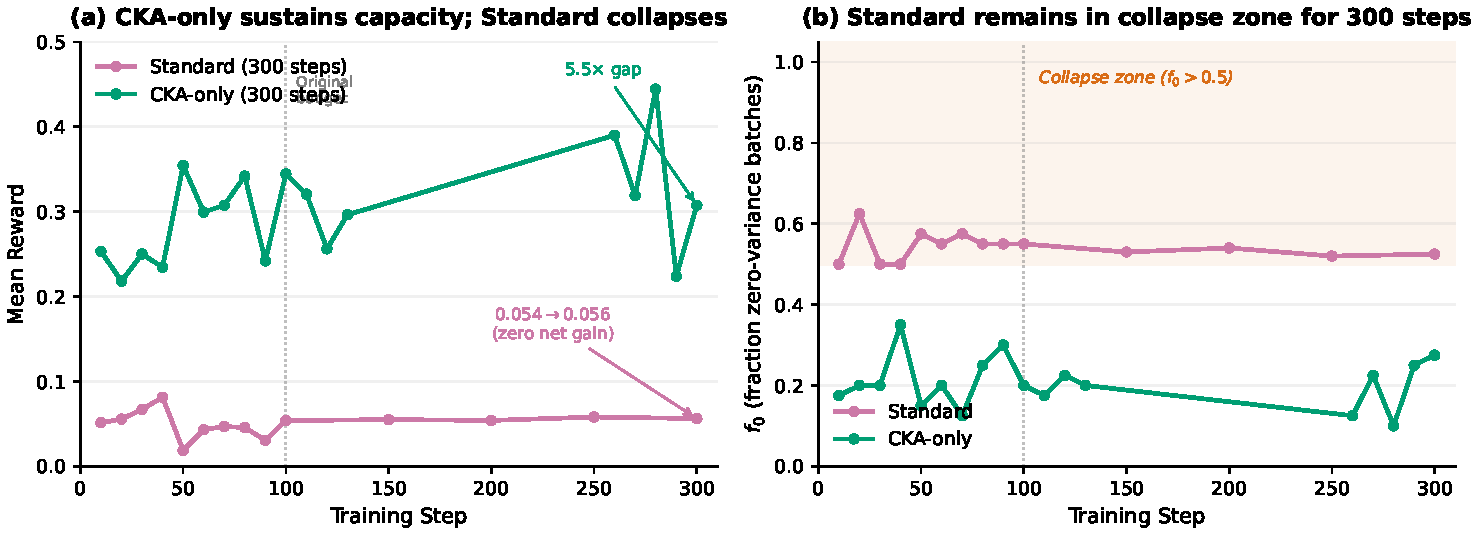
\includegraphics[width=0.85\columnwidth]{figures/paper/fig5_extended_training.pdf}
    \caption{Extended GRPO training (300 steps, 3$\times$ original budget). (a)~Standard reward shows zero net gain (0.054$\to$0.056); CKA-only oscillates in the 0.22--0.44 range with a 5.5$\times$ gap at step 300. (b)~Standard $f_0$ remains in the collapse zone ($>$0.5); CKA-only stays below 0.30.}
    \label{fig:extended_training}
\end{figure}

\section{MATH-500 Out-of-Distribution Evaluation}
\label{sec:appendix_math500}

\begin{table}[h]
\centering
\small
\caption{Out-of-distribution evaluation on MATH-500 ($N{=}500$, greedy decoding, \texttt{max\_new\_tokens=2048}). The recovery capacity spectrum persists across sparsity levels. Reward-accuracy decoupling holds across all completed SFT/GRPO pairs ($|\Delta| \leq 1.2$\,pp).}
\label{tab:math500}
\begin{tabular}{@{}llc@{}}
\toprule
Method & Recovery & MATH-500\,(\%) \\
\midrule
Dense & -- & 53.0 \\
\midrule
\multicolumn{3}{l}{\textit{20\% sparsity}} \\
CKA-only & SFT & 26.8 \\
CKA-only & GRPO & 26.6 \\
\midrule
Standard & SFT & 25.8 \\
\rasp{} & SFT & 22.6 \\
\midrule
\multicolumn{3}{l}{\textit{25\% sparsity}} \\
CKA-only & SFT & 19.2 \\
CKA-only & GRPO & 18.4 \\
\midrule
Standard & SFT & 14.0 \\
Standard & GRPO & 12.8 \\
\bottomrule
\multicolumn{3}{p{0.85\columnwidth}}{\footnotesize Over half of Dense model responses are truncated at 2048 tokens, depressing absolute accuracy (73.6\% at 4096 tokens vs 53.0\% at 2048). All pruned models are evaluated under the same constraint for fair comparison. 20\% SFT/GRPO pairs incomplete due to evaluation failures; available checkpoints reported.}
\end{tabular}
\end{table}


\section{MBPP Code Generation}
\label{sec:appendix_mbpp}

\begin{table}[h]
\centering
\small
\caption{MBPP code generation accuracy ($N{=}374$, greedy decoding). All fine-grained pruning methods converge near a capability floor (${\sim}$75\% code capability loss vs Dense), limiting differentiation (${\sim}$1\,pp range, within stderr). ShortGPT shows a larger GRPO delta ($+$4.01\,pp) but at the 95\% CI boundary (stderr ${\approx}$1.55\,pp).}
\label{tab:mbpp}
\begin{tabular}{@{}lccc@{}}
\toprule
Method & SFT\,(\%) & GRPO\,(\%) & $\Delta$\,(pp) \\
\midrule
Dense & -- & 53.48 & -- \\
\midrule
CKA-only 20\% & 12.83 & 14.17 & $+$1.34 \\
Standard 20\% & 12.03 & 13.10 & $+$1.07 \\
\rasp{} 20\% & 11.76 & 13.10 & $+$1.34 \\
\midrule
ShortGPT 20\%$^\dagger$ & 10.43 & 14.44 & $+$4.01 \\
\bottomrule
\multicolumn{4}{l}{\footnotesize $^\dagger$Depth pruning; removes entire layers.}
\end{tabular}
\end{table}


\section{CKA Scoring Stability}
\label{sec:appendix_cka_stability}

\begin{table}[h]
\centering
\small
\caption{CKA scoring stability across calibration sizes. Spearman $\rho$ between structure rankings produced by different calibration set sizes. High correlation ($\rho \geq 0.964$) indicates that CKA-based scoring is robust to calibration data volume.}
\label{tab:cka_stability}
\begin{tabular}{@{}lcc@{}}
\toprule
Calibration Sizes & Spearman $\rho$ (min) & Spearman $\rho$ (mean) \\
\midrule
256 / 512 / 1024 & 0.964 & 0.979 \\
\bottomrule
\end{tabular}
\end{table}


CKA-based structure rankings are highly stable across calibration data volumes: Spearman $\rho$ between rankings from 256, 512, and 1024 calibration samples ranges from 0.964 to 0.979, indicating that the scoring criterion is not sensitive to calibration set size.

\section{Seed Reproducibility}
\label{sec:appendix_seed}

CKA-only GSM8K accuracy across 3 GRPO seeds: 64.37\% (seed 42), 64.22\% (seed 123), 64.58\% (seed 456), yielding mean 64.39\% $\pm$ 0.19\,pp.
Standard: mean 59.84\% $\pm$ 0.38\,pp across the same 3 seeds.
See Table~\ref{tab:multiseed} for the full summary.

\section{Sparsity Cliff at 30\%}
\label{sec:appendix_sparsity_cliff}

\begin{table}[t]
\centering
\caption{Sparsity cliff at 30\% structured sparsity ($N{=}100$). All tested pruning criteria collapse, with near-zero accuracy and EOS generation rates below 6\%.}
\label{tab:sparsity_cliff}
\begin{tabular}{@{}lcc@{}}
\toprule
Method & Acc.\,(\%) & EOS Rate\,(\%) \\
\midrule
Standard & 4 & 5.5 \\
\rasp{} & 0 & 3.0 \\
CKA-only & 0 & --$^\dagger$ \\
\bottomrule
\multicolumn{3}{@{}l}{\footnotesize $^\dagger$Terminated early after collapse confirmed.}
\end{tabular}
\end{table}


All tested methods collapse at 30\% sparsity: Standard retains 4\% accuracy, \rasp{} and CKA-only reach 0\%.
This capacity threshold, independent of pruning criterion, validates 20\% as the operating point and confirms that the recovery capacity spectrum reflects how methods allocate a limited pruning budget.

\section{Multi-Seed GRPO Results}
\label{sec:appendix_multiseed}

\begin{table}[h]
\centering
\small
\caption{Multi-seed GRPO results on GSM8K ($N{=}1{,}319$). CKA-only and Standard each trained with 3 GRPO seeds (42, 123, 456); pruning calibration and SFT are identical across all runs within each sparsity level.}
\label{tab:multiseed}
\begin{tabular}{@{}llccc@{}}
\toprule
Sparsity & Method & Mean Acc.\,(\%) & Std\,(pp) & Seeds \\
\midrule
\multirow{3}{*}{20\%} & CKA-only & 64.39 & 0.19 & 3 \\
 & Standard & 59.84 & 0.38 & 3 \\
 & \rasp{} & 60.88 & -- & 1 \\
\midrule
\multirow{2}{*}{15\%} & CKA-only & 72.76 & 0.57 & 3 \\
 & Standard & 65.56 & 0.50 & 3 \\
\bottomrule
\end{tabular}
\end{table}

At 20\% sparsity, the 4.55\,pp gap between CKA-only and Standard is robust across seeds, with non-overlapping ranges (CKA-only: 64.22--64.58\%, Standard: 59.44--60.20\%).
Standard shows higher seed variance (0.38\,pp vs 0.19\,pp), consistent with borderline-collapse dynamics where small perturbations produce larger outcome variation.
Note: Standard seed 42 was trained from a separately initialized SFT checkpoint (accuracy 59.21\% vs.\ 59.29\% for seeds 123/456; $\Delta = 0.08$\,pp).
At 15\% sparsity, the gap widens to 7.20\,pp (72.76\% vs 65.56\%, $t{\approx}16.4$, $p{<}0.001$), with non-overlapping ranges (CKA-only: 72.10--73.09\%, Standard: 65.13--65.43\%).

\section{Cross-Sparsity Validation}
\label{sec:appendix_cross_sparsity}

\begin{table}[h]
\centering
\small
\caption{Cross-sparsity validation on DeepSeek-R1-Distill-Qwen-7B. GSM8K accuracy ($N{=}1{,}319$) after SFT warmup and GRPO recovery. 15\% and 20\% GRPO values are mean over 3 seeds (see Tables~\ref{tab:decoupling},~\ref{tab:multiseed}). $^\ddagger$Single seed. Mean $|\Delta| \leq 1$\,pp across all conditions.}
\label{tab:cross_sparsity}
\begin{tabular}{@{}llccc@{}}
\toprule
Sparsity & Method & SFT\,(\%) & GRPO\,(\%) & $\Delta$\,(pp) \\
\midrule
\multirow{2}{*}{15\%} & CKA-only & 72.18 & \textbf{72.76{\scriptsize$\pm$0.57}} & $+$0.58 \\
 & Standard & 66.49 & 65.56{\scriptsize$\pm$0.50} & $-$0.93 \\
\midrule
\multirow{2}{*}{20\%} & CKA-only & 63.91 & 64.39 & $+$0.48 \\
 & Standard & 59.29 & 59.84 & $+$0.55 \\
\midrule
\multirow{2}{*}{25\%$^\ddagger$} & CKA-only & 60.12 & 59.59 & $-$0.53 \\
 & Standard & 50.87 & 51.86 & $+$0.99 \\
\midrule
30\% & All & \multicolumn{3}{c}{Collapse ($\leq$4\%; Table~\ref{tab:sparsity_cliff})} \\
\bottomrule
\end{tabular}
\end{table}

At 15\% sparsity (3-seed mean), the CKA-only advantage widens to $+$7.20\,pp (72.76\% vs 65.56\%), compared to $+$4.55\,pp at 20\%.
CKA-only at 15\% (72.76\%) represents the highest mean accuracy across all experimental conditions, retaining 80.1\% of original dense model performance (90.83\%).
At 25\% sparsity (single seed), Standard's SFT accuracy decline accelerates ($-$7.20\,pp from 15\%$\to$20\%, $-$8.42\,pp from 20\%$\to$25\%), while CKA-only's decline decelerates ($-$8.27\,pp then $-$3.79\,pp).
Reward-accuracy decoupling is preserved ($|\Delta| \leq 1$\,pp for both methods) despite Standard's near-zero peak reward (0.008).

\section{Cross-Architecture Validation}
\label{sec:appendix_cross_arch}

\begin{table}[h]
\centering
\small
\caption{Cross-architecture validation on Qwen2.5-Math-7B~\citep{qwen2.5} at 20\% structured sparsity. Accuracy evaluated on GSM8K ($N{=}200$). Post-SFT reports mean $\pm$ std over multiple SFT runs. EOS rate: fraction of generations that produce a valid end-of-sequence token.}
\label{tab:cross_arch}
\begin{tabular}{@{}lccc@{}}
\toprule
Method & Post-Prune\,(\%) & Post-SFT\,(\%) & EOS Rate\,(\%) \\
\midrule
CKA-only & 1.0 & \textbf{51.50 $\pm$ 3.53} & 27.0 \\
Standard & 18.5 & 21.00 $\pm$ 2.88 & 36.5 \\
\bottomrule
\end{tabular}
\end{table}

CKA-only pruning causes near-total initial damage on Qwen2.5-Math-7B (1.0\% post-prune accuracy vs Standard's 18.5\%), yet SFT recovers CKA-only to 51.50\% while Standard remains at 21.00\%.
This post-prune accuracy reversal provides strong evidence that recovery capacity is shaped by preserved network structure rather than starting accuracy.
EOS rates remain below 40\% for both methods, indicating that SFT warmup is less effective on this architecture; GRPO recovery may yield further improvements but was not run due to compute constraints.

\section{Structural Overlap Analysis}
\label{sec:appendix_overlap}

CKA-only and Standard pruning produce markedly different removal patterns across the 28 layers of DeepSeek-R1-Distill-Qwen-7B at 20\% sparsity.
CKA-only concentrates pruning in early layers (L0--9 account for 72.5\% of removed MLP groups), preserving nearly all structures in later layers (L16--27).
Standard distributes removals more uniformly, pruning substantial numbers of groups in late layers (L16--18, L22, L25--26).

The methods share only partial overlap in which structures they remove.
65 MLP groups are pruned exclusively by CKA-only (retained by Standard), concentrated in L6--9 and L27---structures that gradient importance scores as important but CKA identifies as redundant with neighboring groups.
Conversely, 46+ groups are pruned exclusively by Standard (retained by CKA-only), concentrated in L16--18, L22, and L25--26---structures that gradient importance scores as unimportant but CKA identifies as representationally unique.

This pattern is consistent with the CKA heatmap (Figure~\ref{fig:cka_heatmap}): CKA-only's aggressive early-layer pruning disrupts dense representations (low diagonal CKA, $\mu{=}0.62$) but preserves diverse late-layer pathways, while Standard's uniform pruning maintains dense fidelity ($\mu{=}0.90$) at the cost of removing unique computational pathways in later layers.

\section{KL Divergence During GRPO Training}
\label{sec:appendix_kl}

\begin{figure}[t]
    \centering
    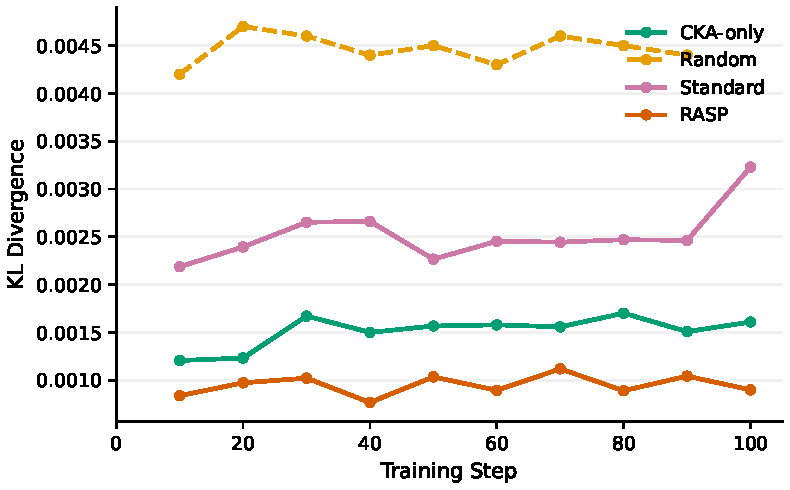
\includegraphics[width=0.75\columnwidth]{figures/paper/fig_appendix_kl.pdf}
    \caption{KL divergence between the policy and reference model during GRPO training. RASP maintains near-zero KL ($<$0.001), consistent with minimal policy movement during collapse. Random shows the highest KL (${\sim}$0.004--0.005), indicating more policy exploration. CKA-only and Standard fall between these extremes.}
    \label{fig:kl_divergence}
\end{figure}
